
\chapter{Methods}

The impact of video games in recent years has increased considerably, which has allowed the emergence of new fields of research. Currently, many studies have established design practices that allow improving the user experience or even using video games as a method to improve educational processes (citation), however, the elements that directly influence the difficulty of the challenges proposed into the virtual universes it is still uncertain. For this reason, we have defined as the main objective of this research, to evaluate and validate some factors within a specific situation, presenting a digital environment that progressively increases its complexity by modifying specific variables.

In this way, a design process has been carried out to establish the main aspects to be integrated into the virtual environment; to later develop the application and obtain relevant information from the user behavior. We have fragmented the latter into two groups: experienced and inexperienced users, thus confirming that the player's experience directly influences their performance (citation).

At the same time reaching the conclusion of adopting as secondary objectives the design of a video game where you can evaluate some of the factors that have a potential relationship with the difficulty. Focusing mainly on the video games platformers type, thinking this one could be the most common type of video game to be previously played by people and tanking into account this type of game has already in the patterns and speed of enemies a potential factors that affect the difficulty of these. The patterns, we will use for this investigation are those that have the x-axis as the main axis, which means horizontal patterns, the in-depth explanation of these patterns will be found later in the design and development section.

For the data collection, we have a secondary objective that is the storage and analysis of the possible dependent variables generated from the interaction of the participants with the proposed virtual environment. The main dependent variable is the minimum distance between the participant's virtual character and the enemies when performing any action, we can understand this in more detail in the design and development section.

\section{Design \& Development}

As previously mentioned, the proposed method is the creation of a platform video game to evaluate the difficulty in two factors, see Figure 2, the first factor is the patterns of the enemies and the second factor is the speed of their movement, within this investigation we will focus specifically on horizontal patterns and these horizontal patterns we will divide it into Patterns with subdivisions at a distance in x (defined by a scalar $\alpha$) and patterns with points of random choice in x (defined by a scalar $\beta$).

\begin{figure}[ht]
    \centering
      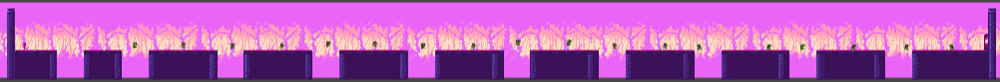
\includegraphics[width=\linewidth]{Figures/completelevel.png}
      \caption{A full view of the level.}
    \label{fig:example}
\end{figure}

what $\alpha$ will show is a series of jumps equivalent to the number of subdivisions in the y-axis, to expand this idea look at figure 3.

\begin{figure}[ht]
    \centering
      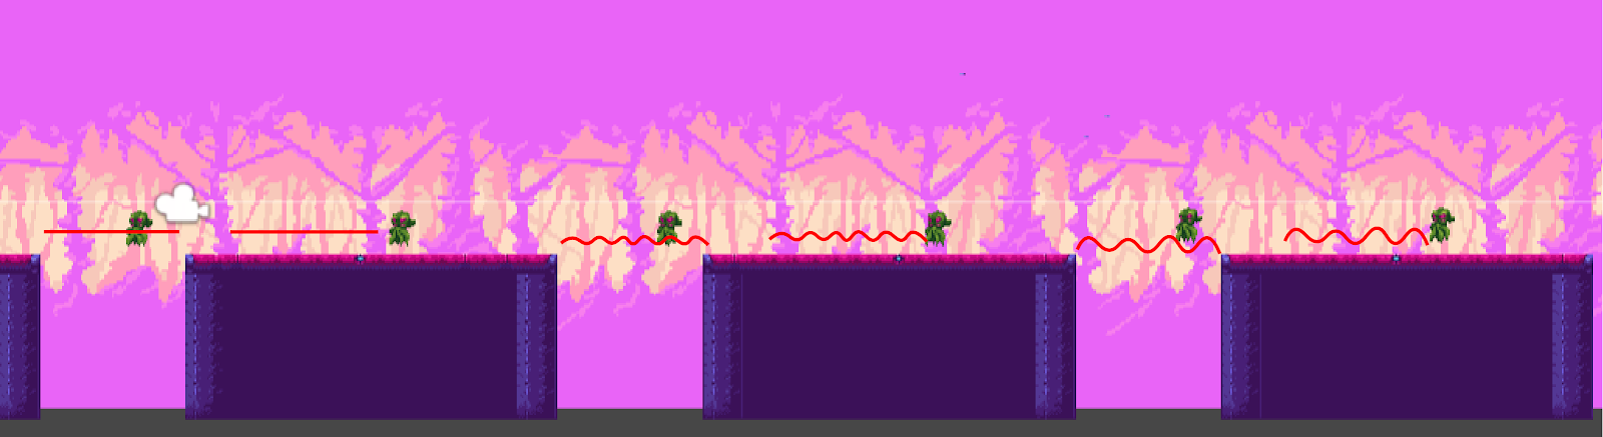
\includegraphics[width=\linewidth]{Figures/alphapath.png}
      \caption{The red lines and curves in the image represent some of the possible $\alpha$, as we can see as more subdivisions it will generate smaller arcs, while with fewer subdivisions it tends to have larger arcs.}
    \label{fig:example}
\end{figure}

On the other hand, the scalar $\beta$ will define the number of possible places to which the enemy can move, e.g. if the number of points or possible places is 4, it means that the enemy, in a random way, will move between those four points; for more information see figure 4.

\begin{figure}[ht]
    \centering
      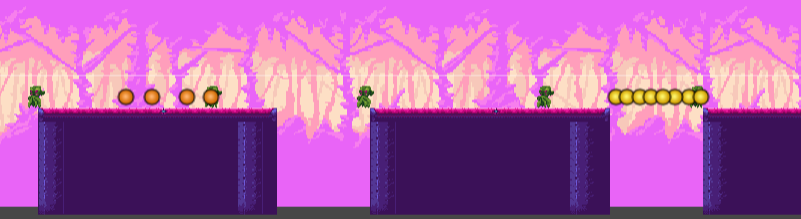
\includegraphics[width=\linewidth]{Figures/betapath.png}
      \caption{The orange and yellow dots in the image represent some of the possible random decision points they have when moving enemies. In the case of oranges $\beta$ = 4 and the case of yellows $\beta$ = 8}
    \label{fig:example}
\end{figure}

A hole (h) parameter has also been included, which evaluates for each $\alpha$ and $\beta$ if there is an added difficulty when integrating a hole; see Figure 5.

\begin{figure}[ht]
    \centering
      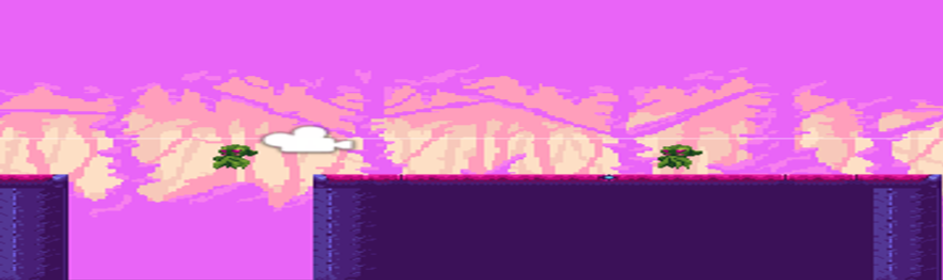
\includegraphics[width=\linewidth]{Figures/holev.png}
      \caption{We can see how these two enemies have a state where there are a hole and another in which it is on a platform, in this case, both enemies have the same pattern $\alpha$ = 0 and $\beta$ = 2 where it will move from one side to the other linearly at x.}
    \label{fig:example}
\end{figure}

As previously mentioned, this virtual environment is developed in Unity 2019.3.06f which is a multiplatform video game engine created by Unity Technologies. In this specific case using the C \# programming language for object-oriented programming. The assets (Tilesets, sprites, and background) come from the asset store of Unity, around this topic a question also arises that will not be answered within this research and is: Does the graphic aspect influence the performance of someone who plays video games?

Talking punctually about the characters in the virtual environment we have these constants:
The maximum movement distance in x that each enemy reaches is 3.2 meters (this measure is understood within the virtual environment). And the maximum movement distance in and having an $\alpha$ of 4 is 0.87 meters.
The minimum distance the user can have with an enemy is when colliding with it and is close to 0.6.
The virtual character has a jump force of 500, thus generating a jump height of 0.5 meters. When you reach the door at the end of this level, reset the level and add one to the speed of the enemies, starting at 1 and achieving a maximum value of 6.

Every time the user's character collides with an enemy, it reappears at a checkpoint that is always in a position after the enemy the user collided with. When reappearing in this position, the character's actions will be disabled for 3 seconds. In case of colliding with the last enemy in the level, this will be the same as the restart of the level and increasing the speed value by 1.

The research question who begins this research is, What are the factors that affect the difficulty of video games for humans? taking into account this question we formalize this hypothesis:

-The combination of the different paths (different $\alpha$ and $\beta$) and the speed is harder than the evaluation of each of these things for separate.
-The holes make easier to avoid the enemies with these two parameters( $\alpha$ and $\beta$)
-A higher $\alpha$ means a lower distance when you execute an action.
-A higher $\beta$ means a lower distance when you execute an action.
-The expected function in this experiment is a decreasing function for each of the possible cases, validating the other hypothesis above.
-It is more difficult a higher $\alpha$ than a higher $\beta$.

Expecting a decreasing function on some of these graphs as the main result, To know a decreasing function f is a function such that increasing the independent variable ($\alpha$, $\beta$, h, speed) x decreases the dependent variable (Distance) y. A function f is decreasing if for every point x in the domain the derivative is negative, that is f '(x) $\succeq$ 0. We will touch on this topic in greater depth in the section Procedures used to obtain data and results.

\section{Experiment Design - Set-Up}

To develop a good experiment several measures are proposed, the experiment will take place in a closed space where distractions can be avoided during experimentation time.

The interface to play is the computer keyboard, using the right and left arrows for movement into the virtual environment, and the space bar to jump. The in-game camera moves with the character as can be seen in Figure 6.
In order to reach the conclusion of this interface, it was discussed in this regard and the result of the said discussion was the use of a simple interface, of daily use and that is known by the majority of participants. Also thought in case of carrying out the tests on several computers and in this way not having the need to build multiple interfaces since the testing time is limited.

\begin{figure}[ht]
    \centering
      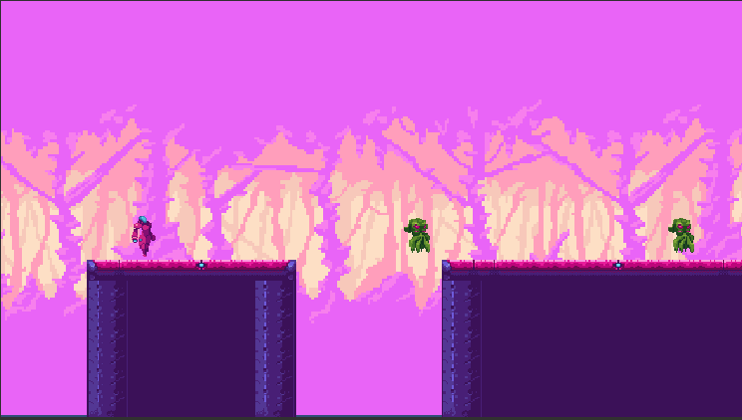
\includegraphics[width=\linewidth]{Figures/cameraview.png}
      \caption{The visualization of the camera, this is how the participant will be able to appreciate the virtual environment.}
    \label{fig:example}
\end{figure}

In this space we mention before we gonna have: a computer, a screen, headphones for the reproduction of the game's audio since the effect of music in video games has been studied and has an effect (for more information cite paper), a table, a chair and a person doing a follow-up in case of any doubt. The participant must read the instructions at the beginning of the game and play trying to achieve their best performance (ensure that the minimum distance between the virtual character and the enemies is the maximum possible).
At the end of the game, the participant can be able to read and sign the terms of use of their data and a short survey in which they will respond to ensure greater reliability in the data obtained, in addition to having information that may be useful for other possible research.

\section{Procedures used to obtain data and results}
To obtain data as previously mentioned, The plan is saving the minimum distances of each performance (the actions between the virtual character and the enemies into the virtual environment), saving this information in a Json, a simple text format for the exchange of data. Saving in this format for each participant an ID and the 18 possible minimum distances for each level, building the Json structure seen in Figure 7.

The expected results, as previously mentioned the graphs could have the behavior of the decreasing functions, the expected results would be for every pattern with a lower $\alpha$ (fewer subdivisions more height) and/or a greater $\beta$ (more points decision or movement) and a higher speed the minimum distance is getting smaller, thus showing that the difficulty to achieve high results is greater.

\begin{figure}[ht]
    \centering
      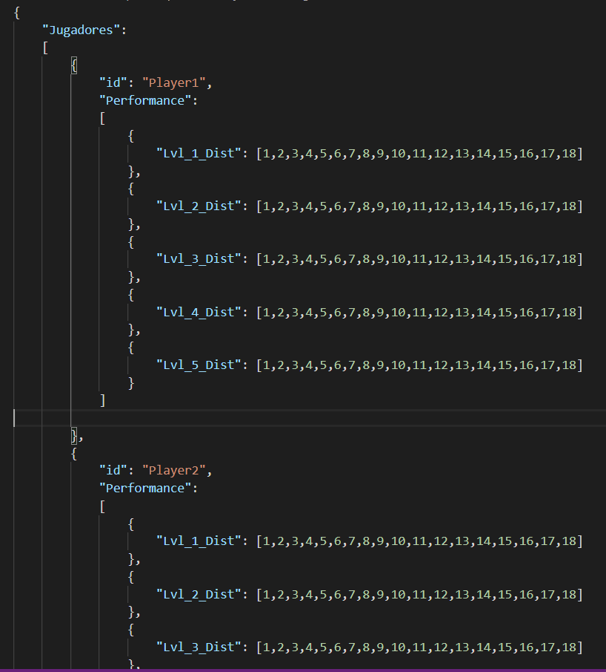
\includegraphics[width=\linewidth]{Figures/json.png}
      \caption{Data saving structure, JSON.}
    \label{fig:example}
\end{figure}

\newpage


